% Figure macros. Diagrams are TikZ (figures/fig_*.tex); data figures are PDFs drawn by
% code/figures/e25_figures.py (E25_*) and code/figures/paper_figures.py via E18 (E18_frontier).

\newcommand{\FigurePath}{%
\begin{figure*}[t]
\centering
% Figure 1: the research path, five stages in one row (TikZ, monochrome). Input by \FigurePath in figs.tex.
% Box width 25.4 mm text + 2 x 1.6 mm padding; four 3.6 mm gaps: 5 x 28.6 + 4 x 3.6 = 157.4 mm (text width 160 mm).
\begin{tikzpicture}[
  font=\scriptsize,
  stage/.style={draw, rounded corners=1.5pt, align=left, text width=25.4mm, inner xsep=1.6mm, inner ysep=1.8pt,
                anchor=north west, minimum height=34mm},
  arr/.style={-{Stealth[length=3.5pt]}, thick},
]
\def\gap{32.2mm}
\node[stage, fill=black!4] (s1) at (0,0) {%
  \textbf{1\enspace What limits a\\\phantom{1\enspace}classifier?}\\[1pt]
  {\itshape E0--E13, \S\ref{sec:classifier}}\\[2pt]
  Hierarchies, experts, losses and soups fail on DeBERTa. Swapping only the backbone for Qwen3-8B: +0.092 per model, 10/10 seeds.\\[2pt]
  $\Rightarrow$ It \emph{ranks} better than it decides: top-3 holds an acceptable label for 93\%.};
\node[stage] (s2) at (\gap,0) {%
  \textbf{2\enspace Can a larger model\\\phantom{2\enspace}choose among them?}\\[1pt]
  {\itshape E14--E18, \S\ref{sec:cascade}}\\[2pt]
  A 27B LLM picks among M1's top 4 for the 30\% least confident items; one distilled student replaces 10 seeds at a quarter of the GPU time.\\[2pt]
  $\Rightarrow$ The headline is one favourable draw: is the gain real?};
\node[stage, fill=black!4] (s3) at (2*\gap,0) {%
  \textbf{3\enspace Which gains\\\phantom{3\enspace}survive?}\\[1pt]
  {\itshape E19--E23, \S\ref{sec:robust}}\\[2pt]
  Routing and fusion ablations, option order, distillation controls: 0.650 \Stwo{}, frozen.\\[2pt]
  $\Rightarrow$ Its parts are not new, and relevance barely predicts errors: what does it measure?};
\node[stage] (s4) at (3*\gap,0) {%
  \textbf{4\enspace Is evasion in the\\\phantom{4\enspace}question or the speaker?}\\[1pt]
  {\itshape E24--E25, \S\ref{sec:measure}}\\[2pt]
  Labels move with the question; the instrument reads it causally. In the President's role, LLMs answer directly what Presidents answered directly.\\[2pt]
  $\Rightarrow$ It needs the whole answer and a fine-tuned model: no shortcut.};
\node[stage, fill=black!4] (s5) at (4*\gap,0) {%
  \textbf{5\enspace Can it be made\\\phantom{5\enspace}cheaper?}\\[1pt]
  {\itshape E26, \S\ref{sec:precision}}\\[2pt]
  FP8 is not faster as implemented and costs M1 0.045; the cascade loses 0.003, within its own noise.\\[2pt]
  $\Rightarrow$ Future work: fused kernels, QLoRA.};
\foreach \a/\b in {s1/s2, s2/s3, s3/s4, s4/s5}
  \draw[arr] ($(\a.north east)+(0,-4.5mm)$) -- ($(\b.north west)+(0,-4.5mm)$);
\end{tikzpicture}

\caption{The research path. Each stage answers one question, and its answer (last line of each box) raises the next. Experiment ids refer to the ledger in Appendix~\ref{sec:ledger}.}
\label{fig:path}
\end{figure*}}

\newcommand{\FigureSystem}{%
\begin{figure*}[t]
\centering
% Figure 2: the whole system in one picture (TikZ, monochrome, within the 160 mm text width). Input by \FigureSystem.
% Three columns: (left) what is trained or fitted, and on which data; (middle) the cascade, which after E23 is the
% frozen instrument; (right) how the instrument is used in E25/E26. Each side box sits level with the stage it
% feeds, so every arrow is straight. Widths: side 38 mm, middle 54 mm, gaps 7 mm (frames span ~153 mm).
\begin{tikzpicture}[
  font=\scriptsize,
  box/.style={draw, rounded corners=1.5pt, align=center, inner xsep=2pt, inner ysep=2pt},
  side/.style={box, align=left, text width=38mm},
  arr/.style={-{Stealth[length=3.2pt]}, thin},
  head/.style={font=\footnotesize\bfseries, anchor=south, inner sep=2pt, text height=1.7ex, text depth=0.4ex},
  frame/.style={draw, densely dotted, rounded corners=3pt, inner sep=2mm},
]
% ---------------- middle column: the cascade ----------------
\node[box, fill=black!6, text width=54mm, anchor=north] (in) at (80mm,0) {%
  \textbf{Input} $x$:\enspace sub-question $q$,\enspace full question $Q$,\enspace answer $a$};
\node[box, text width=54mm, anchor=north] (m1) at ($(in.south)+(0,-9mm)$) {%
  \textbf{M1}\enspace Qwen3-8B + LoRA, 10 seeds $\rightarrow$ mean $\bar p(c \mid x)$\\
  candidates $C(x)$ = top 4;\enspace uncertainty $u(x)$};
\node[box, text width=54mm, anchor=north] (m2) at ($(m1.south)+(0,-5mm)$) {%
  \textbf{M2}\enspace defer iff $u(x) \ge \theta$\enspace(the 30\% least confident)};
\node[box, text width=19mm, anchor=north west] (keep) at ($(m2.south west)+(0,-6mm)$) {%
  \textbf{Keep M1}\\ $\arg\max_c \bar p / \pi_c^{\tau_1}$};
\node[box, text width=31mm, anchor=north east] (m3) at ($(m2.south east)+(0,-6mm)$) {%
  \textbf{M3}\enspace Qwen3.8-27B\\ picks one letter in $C(x)$;\\
  $q$ over 4 option orders,\\ fused with $\bar p$};
\node[box, fill=black!6, text width=54mm, anchor=north] (out) at ($(m2.south)+(0,-23mm)$) {%
  \textbf{Subtask 2} evasion type (9) $\rightarrow$ \textbf{Subtask 1} level (3)};
\draw[arr] (in) -- (m1);
\draw[arr] (m1) -- (m2);
\draw[arr] (m2.south -| keep.north) -- node[right, inner sep=1pt] {no} (keep.north);
\draw[arr] (m2.south -| m3.north) -- node[right, inner sep=1pt] {yes} (m3.north);
\draw[arr] (keep.south) -- (keep.south |- out.north);
\draw[arr] (m3.south) -- (m3.south |- out.north);

% ---------------- left column: training and fitting ----------------
\node[side, anchor=east] (a1) at ($(m1.west)+(-7mm,0)$) {%
  \textbf{Train} 10 LoRA seeds on 3,103 train rows, 12 epochs; epoch chosen on the train slice};
\node[side, anchor=east] (a2) at ($(m2.west)+(-7mm,-1.5mm)$) {%
  \textbf{Calibrate} on the train slice (345 rows): temperature, top-4 rule, threshold $\theta$};
\node[side, anchor=east] (a5) at ($(keep.west)+(-7mm,0)$) {%
  \textbf{Fit on dev by nested CV:} $\tau_1$ for kept items; $\lambda, \tau$ of the fusion};
\node[side, anchor=north east, dashed] (a4) at ($(a5.south east)+(0,-2.5mm)$) {%
  \textbf{M4}\enspace M3 labels every train row's cross-fitted top 4; one student on $\tfrac12$gold${}+\tfrac12 q$ replaces M1's seeds};
\draw[arr] (a1.east) -- (m1.west);
\draw[arr] (a2.east) -- (a2.east -| m2.west);
\draw[arr] (a5.east) -- (keep.west);

% ---------------- right column: using the frozen instrument ----------------
\node[side, anchor=north west] (c1) at ($(in.north east)+(7mm,0)$) {%
  \textbf{E25} new inputs, same instrument:\\
  (a) each answer with its own, an unrelated or no question;
  (b) LLM answers to the Presidents' questions in four roles;
  (c) the first 25/50/75\% of each answer};
\node[side, anchor=west, dashed] (c4) at ($(m2.east)+(7mm,1.5mm)$) {%
  \textbf{E26} M1 run in FP8 or NF4 instead of 16-bit};
\node[side, anchor=west] (c5) at ($(out.east)+(7mm,0)$) {%
  \textbf{Measure} Clear-Reply share, label persistence, odds ratios, agreement};
\draw[arr] (c1.west |- in.east) -- (in.east);
\draw[arr, densely dashed] (c4.west) -- ++(-3.5mm,0) |- (m1.east);
\draw[arr] (out.east) -- (c5.west);
% ---------------- frames: one shared top (the input) and bottom (the lowest box) ----------------
\coordinate (top) at (in.north);
\coordinate (bot) at (c5.south);
\node[frame, fit=(a1)(a4)(a1.west |- top)(a1.west |- bot)] (train) {};
\node[frame, fit=(in)(out)(in.west |- bot)] (cascade) {};
\node[frame, fit=(c1)(c5)(c1.east |- top)(c1.east |- bot)] (use) {};
\node[head] at (train.north) {Training and fitting};
\node[head] at (cascade.north) {The cascade = the instrument};
\node[head] at (use.north) {Using the frozen instrument};
\end{tikzpicture}

\caption{The whole system. Left: what is trained or fitted, and on which data. Middle: the cascade, frozen after E23 as the \emph{instrument}. Right: its use, on new inputs (E25) or with a lower-precision M1 (E26), always with the same settings.}
\label{fig:system}
\end{figure*}}

\newcommand{\FigureAudit}{%
\begin{figure*}[t]
\centering
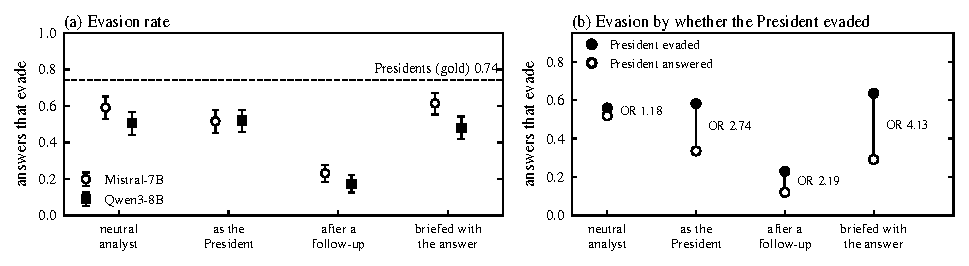
\includegraphics[width=\textwidth]{figures/fig_e25_audit.pdf}
\caption{E25b, labelled by the frozen instrument. (a)~Share of LLM answers that evade, with 95\% cluster-bootstrap intervals (dashed line: the Presidents' gold rate). (b)~The association as plain rates: the share of answers that evade where the President evaded (filled) and where the President answered (open), pooled over the two models, with the odds ratio beside each pair.}
\label{fig:audit}
\end{figure*}}

\newcommand{\FigureSwap}{%
\begin{figure*}[t]
\centering
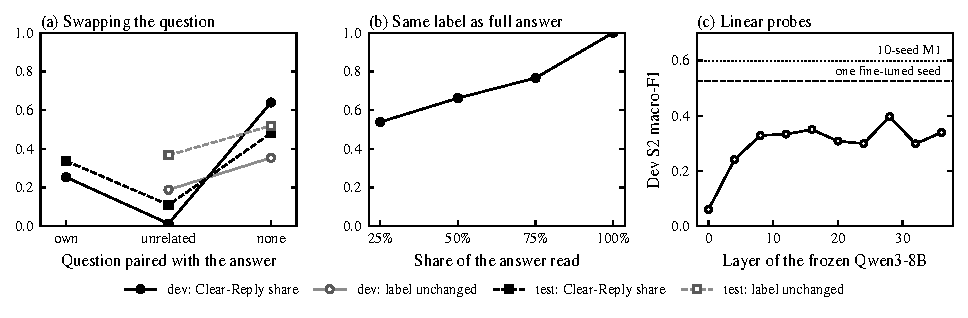
\includegraphics[width=\textwidth]{figures/fig_e25_swap_probe.pdf}
\caption{E25a, c and d. (a)~Each answer paired with its own question, a question from another interview, or none. ``Label unchanged'' is the share of items keeping their own-question label. (b)~Agreement of the label on the first 25/50/75\% of the answer with the full-answer label (dev). (c)~Linear probes on every fourth layer of the frozen Qwen3-8B-Base.}
\label{fig:swap}
\end{figure*}}

\newcommand{\FigureStageOne}{%
\begin{figure*}[t]
\centering
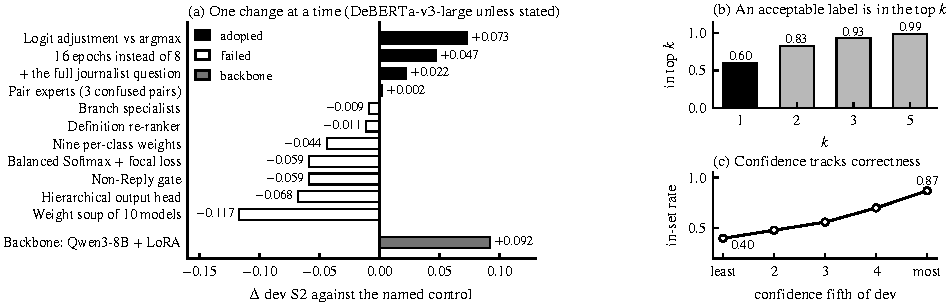
\includegraphics[width=\textwidth]{figures/fig_stage1.pdf}
\caption{Stage~1 on dev \Stwo{}. (a)~Each change against its named control (E0--E13): per model for training and input changes, per system for the rest. (b, c)~The Qwen3-8B classifier ranks better than it decides, and correctness rises with confidence (3 epochs, seeds 0--2).}
\label{fig:stage1}
\end{figure*}}

\newcommand{\FigureFrontier}{%
\begin{figure}[t]
\centering
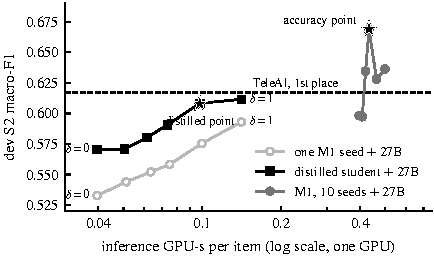
\includegraphics[width=\columnwidth]{figures/fig_frontier.pdf}
\caption{The cascade on dev: \Stwo{} against inference GPU-s per item, for deferral rates $\delta = 0, 0.1, 0.2, 0.3, 0.5, 1$ (left to right on each curve, first scoring, one option order). All times are on one GPU (Appendix~\ref{sec:impl}). TeleAI's GPU time is not published.}
\label{fig:frontier}
\end{figure}}

\newcommand{\FigureStageThree}{%
\begin{figure*}[t]
\centering
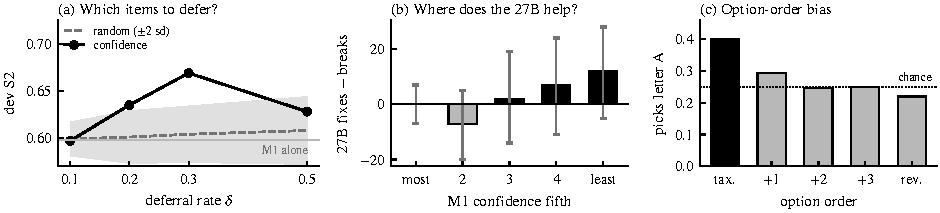
\includegraphics[width=\textwidth]{figures/fig_stage3.pdf}
\caption{Stage~3 (E19--E22), registered tests of the Stage~2 result. (a)~Confidence routing against 200 random routings. (b)~Net fixes of the 27B by M1's confidence, on 1,067 leak-free training rows. (c)~How often the 27B picks the first option, by order.}
\label{fig:stage3}
\end{figure*}}

\newcommand{\FigureRelation}{%
\begin{figure}[t]
\centering
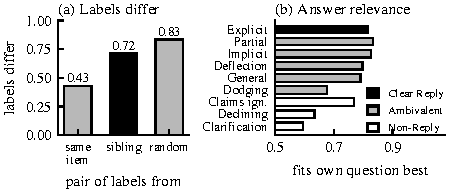
\includegraphics[width=\columnwidth]{figures/fig_relation.pdf}
\caption{Evasion is a relation (E24). (a)~Share of dev label pairs from two annotators that differ: same item, two sub-questions of one answer, random items. (b)~Share of three random questions under which the answer is less likely than under its own, by gold label (train): Partial, Implicit, Deflection and General answers are as relevant as Explicit ones.}
\label{fig:relation}
\end{figure}}

\newcommand{\FigurePrecision}{%
\begin{figure}[t]
\centering
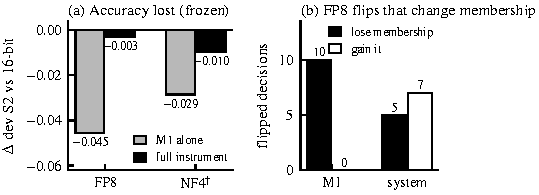
\includegraphics[width=\columnwidth]{figures/fig_precision.pdf}
\caption{E26 on dev, each format against 16-bit on the same GPU type. (a)~\Stwo{} lost, both with frozen parameters. (b)~FP8 flips that change reference-set membership. $^{\dagger}$Lower bound: 27B records missing for 60 NF4 items.}
\label{fig:precision}
\end{figure}}
